% What each ASM rule fires on: four plan-view panels for docs/adk/03_asm_rules.rst.
% Red geometry is what lands in the .lyrdb report; green geometry is deliberately legal.
\documentclass[border=4pt]{standalone}
\usepackage{tikz}
\usetikzlibrary{arrows.meta, calc}
\usepackage[T1]{fontenc}
\usepackage{lmodern}

\definecolor{IHPfg}{RGB}{0,80,139}
\definecolor{IHPaccent}{RGB}{109,112,114}
\definecolor{cFlag}{RGB}{210,80,80}
\definecolor{cLegal}{RGB}{65,155,75}
\definecolor{cGap}{RGB}{200,140,40}

\begin{document}
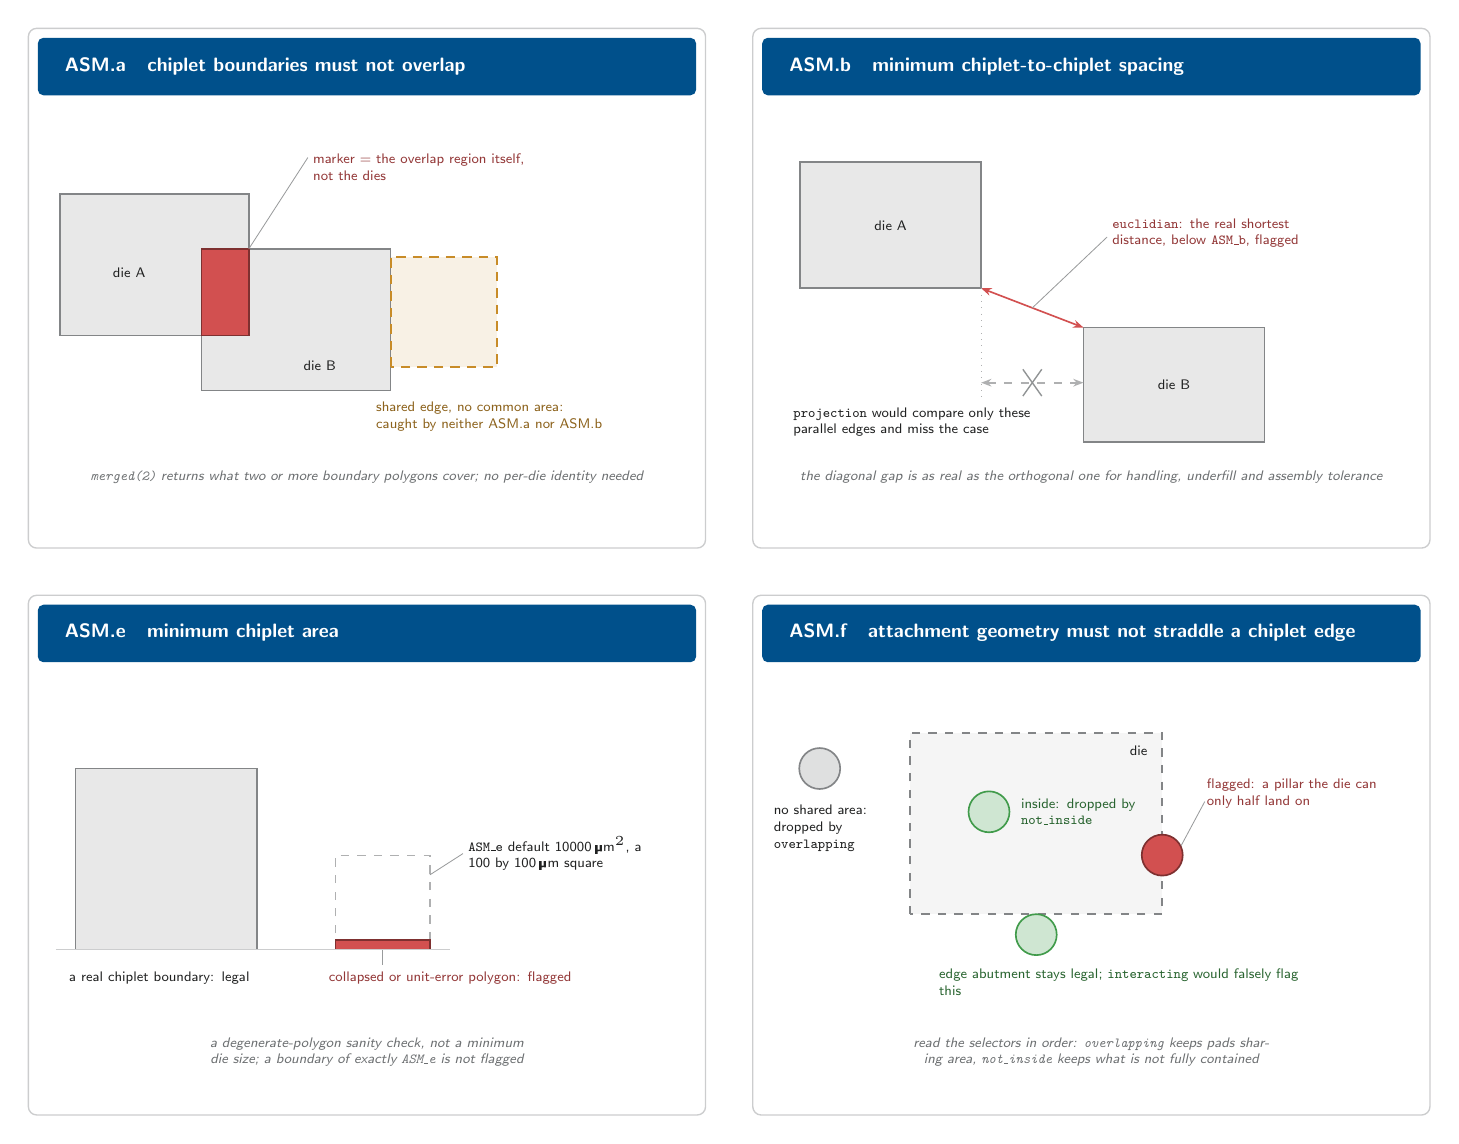
\begin{tikzpicture}[
    >=Stealth,
    adkpanel/.style={
        rounded corners=3pt, draw=IHPaccent!35, line width=0.5pt
    },
    adkbar/.style={
        rounded corners=2pt, fill=IHPfg
    },
    adktitle/.style={
        font=\sffamily\scriptsize\bfseries, text=white, anchor=west
    },
    adkdie/.style={
        fill=IHPaccent!16, draw=IHPaccent!85, line width=0.6pt
    },
    adklbl/.style={
        font=\sffamily\tiny, text=IHPaccent!30!black, align=left, inner sep=0.6mm
    },
    adkred/.style={
        font=\sffamily\tiny, text=cFlag!70!black, align=left, inner sep=0.6mm
    },
    adkgreen/.style={
        font=\sffamily\tiny, text=cLegal!65!black, align=left, inner sep=0.6mm
    },
    adkgap/.style={
        font=\sffamily\tiny, text=cGap!70!black, align=left, inner sep=0.6mm
    },
    adkcap/.style={
        font=\sffamily\tiny\itshape, text=IHPaccent, align=center, inner sep=0.6mm
    },
    adkleader/.style={
        draw=IHPaccent!70, line width=0.3pt
    },
    adkdim/.style={
        {Stealth[length=1.3mm]}-{Stealth[length=1.3mm]}, line width=0.6pt
    },
    adksketch/.style={yshift=-3mm}
]

% =====================================================================
% PANEL a  (top left)
% =====================================================================
\begin{scope}[shift={(0,7.2)}]
  \draw[adkpanel] (0,0) rectangle (8.6,6.6);
  \fill[adkbar] (0.12,5.75) rectangle (8.48,6.48);
  \node[adktitle] at (0.34,6.12) {ASM.a\quad chiplet boundaries must not overlap};

  \begin{scope}[adksketch]
    % two overlapping dies
    \draw[adkdie] (0.40,3.00) rectangle (2.80,4.80);
    \draw[adkdie] (2.20,2.30) rectangle (4.60,4.10);
    \fill[cFlag] (2.20,3.00) rectangle (2.80,4.10);
    \draw[cFlag!60!black, line width=0.6pt] (2.20,3.00) rectangle (2.80,4.10);
    \node[adklbl, anchor=center] at (1.28,3.80) {die A};
    \node[adklbl, anchor=center] at (3.70,2.62) {die B};

    % callout on the overlap marker
    \draw[adkleader] (2.80,4.10) -- (3.55,5.26);
    \node[adkred, anchor=west, text width=45mm] at (3.55,5.14)
      {marker = the overlap region itself,\\not the dies};

    % edge-abutting third die: passes, but only because merged semantics
    % fuses the two boundaries. Neither ASM.a nor ASM.b sees it.
    \draw[fill=cGap!12, draw=cGap, line width=0.7pt, dashed,
          dash pattern=on 1.2mm off 0.9mm]
      (4.60,2.60) rectangle (5.95,4.00);
    \node[adkgap, anchor=north west, text width=41mm] at (4.35,2.22)
      {shared edge, no common area:\\caught by neither ASM.a nor ASM.b};
  \end{scope}

  \node[adkcap, anchor=north, text width=80mm] at (4.30,1.05)
    {\texttt{merged(2)} returns what two or more boundary polygons cover;
     no per-die identity needed};
\end{scope}

% =====================================================================
% PANEL b  (top right)
% =====================================================================
\begin{scope}[shift={(9.2,7.2)}]
  \draw[adkpanel] (0,0) rectangle (8.6,6.6);
  \fill[adkbar] (0.12,5.75) rectangle (8.48,6.48);
  \node[adktitle] at (0.34,6.12) {ASM.b\quad minimum chiplet-to-chiplet spacing};

  \begin{scope}[adksketch]
    % two diagonally offset dies, nearest corners facing each other
    \draw[adkdie] (0.60,3.60) rectangle (2.90,5.20);
    \draw[adkdie] (4.20,1.65) rectangle (6.50,3.10);
    \node[adklbl, anchor=center] at (1.75,4.40) {die A};
    \node[adklbl, anchor=center] at (5.35,2.38) {die B};

    % the euclidian corner-to-corner distance
    \draw[adkdim, color=cFlag] (2.90,3.60) -- (4.20,3.10);
    \draw[adkleader] (3.55,3.35) -- (4.50,4.25);
    \node[adkred, anchor=west, text width=38mm] at (4.50,4.30)
      {\texttt{euclidian}: the real shortest\\distance, below \texttt{ASM\_b},
       flagged};

    % what projection would have compared
    \draw[IHPaccent!55, line width=0.3pt, dotted] (2.90,3.60) -- (2.90,2.20);
    \draw[adkdim, color=IHPaccent!55, dashed] (2.90,2.40) -- (4.20,2.40);
    \draw[IHPaccent!75, line width=0.5pt] (3.43,2.23) -- (3.67,2.57);
    \draw[IHPaccent!75, line width=0.5pt] (3.67,2.23) -- (3.43,2.57);
    \node[adklbl, anchor=north west, text width=32mm] at (0.45,2.15)
      {\texttt{projection} would compare only these parallel edges and miss
       the case};
  \end{scope}

  \node[adkcap, anchor=north, text width=80mm] at (4.30,1.05)
    {the diagonal gap is as real as the orthogonal one for handling,
     underfill and assembly tolerance};
\end{scope}

% =====================================================================
% PANEL e  (bottom left)
% =====================================================================
\begin{scope}[shift={(0,0)}]
  \draw[adkpanel] (0,0) rectangle (8.6,6.6);
  \fill[adkbar] (0.12,5.75) rectangle (8.48,6.48);
  \node[adktitle] at (0.34,6.12) {ASM.e\quad minimum chiplet area};

  \begin{scope}[adksketch]
    % a healthy boundary, on the common baseline
    \draw[adkdie] (0.60,2.40) rectangle (2.90,4.70);
    \node[adklbl, anchor=north west, text width=30mm] at (0.45,2.18)
      {a real chiplet boundary: legal};

    % the ASM_e reference square, behind the sliver
    \draw[IHPaccent!55, line width=0.4pt, dashed] (3.90,2.40) rectangle (5.10,3.60);
    \draw[adkleader] (5.10,3.35) -- (5.52,3.62);
    \node[adklbl, anchor=west, text width=25mm] at (5.52,3.62)
      {\texttt{ASM\_e} default 10000\,\textmu m$^2$, a 100 by 100\,\textmu m
       square};

    % the collapsed sliver
    \fill[cFlag] (3.90,2.40) rectangle (5.10,2.52);
    \draw[cFlag!60!black, line width=0.5pt] (3.90,2.40) rectangle (5.10,2.52);
    \draw[adkleader] (4.50,2.40) -- (4.50,2.20);
    \node[adkred, anchor=north west, text width=33mm] at (3.75,2.18)
      {collapsed or unit-error polygon: flagged};

    % common baseline
    \draw[IHPaccent!35, line width=0.3pt] (0.35,2.40) -- (5.35,2.40);
  \end{scope}

  \node[adkcap, anchor=north, text width=80mm] at (4.30,1.05)
    {a degenerate-polygon sanity check, not a minimum die size;
     a boundary of exactly \texttt{ASM\_e} is not flagged};
\end{scope}

% =====================================================================
% PANEL f  (bottom right)
% =====================================================================
\begin{scope}[shift={(9.2,0)}]
  \draw[adkpanel] (0,0) rectangle (8.6,6.6);
  \fill[adkbar] (0.12,5.75) rectangle (8.48,6.48);
  \node[adktitle] at (0.34,6.12)
    {ASM.f\quad attachment geometry must not straddle a chiplet edge};

  \begin{scope}[adksketch]
    % the die, dashed boundary, very light fill
    \fill[IHPaccent!7] (2.00,2.85) rectangle (5.20,5.15);
    \draw[IHPaccent!85, line width=0.6pt, dashed] (2.00,2.85) rectangle (5.20,5.15);
    \node[adklbl, anchor=north east] at (5.08,5.05) {die};

    % 1. fully inside
    \fill[cLegal!25] (3.00,4.15) circle (0.26);
    \draw[cLegal, line width=0.6pt] (3.00,4.15) circle (0.26);
    \node[adkgreen, anchor=west, text width=17mm] at (3.34,4.15)
      {inside: dropped by \texttt{not\_inside}};

    % 2. no shared area at all
    \fill[IHPaccent!22] (0.85,4.70) circle (0.26);
    \draw[IHPaccent!85, line width=0.6pt] (0.85,4.70) circle (0.26);
    \node[adklbl, anchor=north west, text width=18mm] at (0.20,4.30)
      {no shared area: dropped by \texttt{overlapping}};

    % 3. straddling the right edge
    \fill[cFlag] (5.20,3.60) circle (0.26);
    \draw[cFlag!60!black, line width=0.6pt] (5.20,3.60) circle (0.26);
    \draw[adkleader] (5.44,3.72) -- (5.74,4.28);
    \node[adkred, anchor=west, text width=25mm] at (5.70,4.38)
      {flagged: a pillar the die can only half land on};

    % 4. edge abutment, zero common area
    \fill[cLegal!25] (3.60,2.59) circle (0.26);
    \draw[cLegal, line width=0.6pt] (3.60,2.59) circle (0.26);
    \node[adkgreen, anchor=north west, text width=46mm] at (2.30,2.22)
      {edge abutment stays legal; \texttt{interacting} would falsely flag this};
  \end{scope}

  \node[adkcap, anchor=north, text width=80mm] at (4.30,1.05)
    {read the selectors in order: \texttt{overlapping} keeps pads sharing area,
     \texttt{not\_inside} keeps what is not fully contained};
\end{scope}

\end{tikzpicture}
\end{document}
